\subsection{Frameworks}
\label{subsec:frameworks}


%1. I40 and IIC definition
%2. koloss industries clustering 
%3. what statistcs do we base our categorisation on
%4. where do you see yourself model (aka early adopter etc)

Both the industry and the academic world offer a variety of frameworks, concepts, consulting services and guidelines for businesses, institutions and even cities to employ to optimize their utility from the Digital Transformation.
We focused our attention on frameworks that are applicable to a variety of sections to ensure we define recommendations applicable to businesses independent of region, industry or size. 
We chose four frameworks as applicable to most industries and want to summarize them in the following chapter.

\subsubsection{Industrie 4.0}
The German Industrie 4.0 initiative was created by the German government to improve Germany's economical position in the global market. According to the \emph{Plattform Industrie 4.0}, I4.0 is a specialization of the \emph{Internet of Things and Services} and applies to a subset of all industries, mainly focused on industrial production and manufacturing
\cite[p.41]{umsetzungsstrategie:2015}. Although it is specifically focused on the manufacturing section, it is the most comprehensive initiative we found involving BITKOM e.V., VDMA e.V. and ZVEI e.V., three industrial associations representing IT, electronics and digital economy in Germany \cite{zveimembers:2016, vdmamembers:2016, bitkommembers:2016}. The initiative offers both recommendations and best practices for individual organizations \cite[p.40ff.]{umsetzungsstrategie:2015} as well as describing the strategic plan of progressing the \ac{I4.0} on a national level for the German government \cite[p.15ff.]{umsetzungsstrategie:2015}. It therefore offers a wide range of both high level overviews all the way do very detailed implementation advise on the factory floor.
 The following list summarizes the core goals \cite[p.8]{umsetzungsstrategie:2015}. \footnote{It should be noted that only some of these goals are relevant to individual businesses trying to improve their strategy while others are global environmental necessities. Those that require action of individual businesses are marked with an (X).}

\begin{itemize}
	\item  Standardization (X)
	\item  Reducing of complexity (X)
	\item  Wide band infrastructure
	\item  Security (X)
	\item  Work culture and organization (X)
	\item  Education
	\item  Legal constraints (X)
	\item  Efficiency (X)
\end{itemize}
\footnote{The communication infrastructure as well as education have been excluded under the assumption that they are inputs that are typically not produced by a business itself but rather acquired externally.}

The I4.0 initiative offers several artifacts to support organizations in the transition to a digitalized organization as well as to facilitate the coordination between organizations and industries in researching and developing standards and technologies. 

The most prominent framework is the \ac{RAMI} which has been created as a guideline to avoid definition of multiple, redundant and conflicting standards and communication strategies \cite[p. 41]{umsetzungsstrategie:2015}.

\begin{figure}[H]
\centering
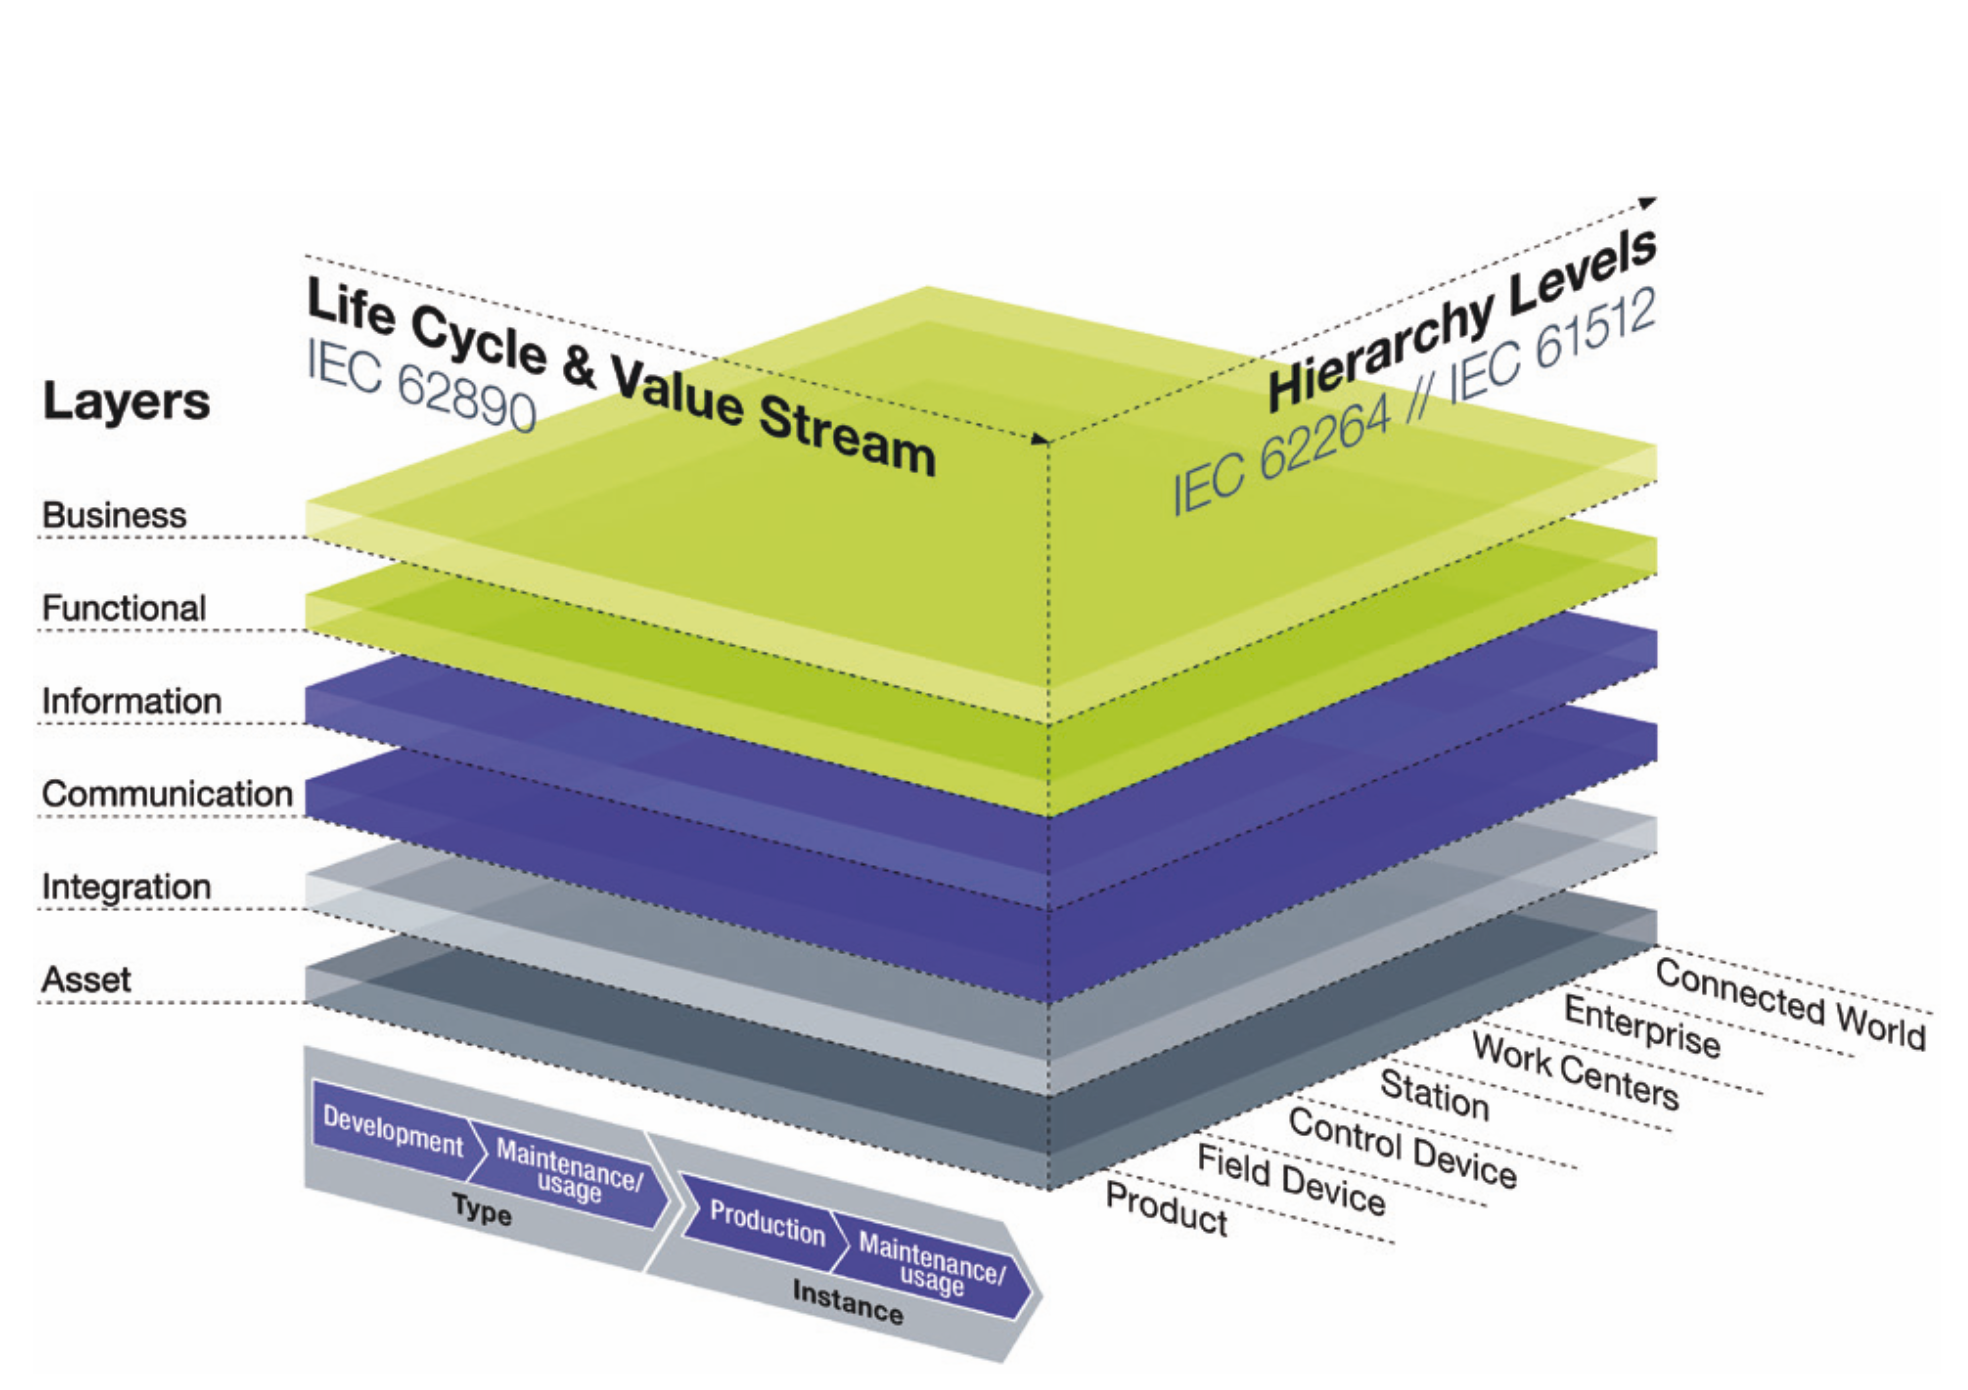
\includegraphics[width=1\columnwidth]{images/RAMI}
\caption{\ac{RAMI} from \citeauthor{umsetzungsstrategie:2015}}
\end{figure}

The \ac{RAMI} framework focuses on three dimensions \emph{layers, Life Cycle \& Value Stream} and \emph{Hierarchy Levels}. By layers, the framework takes reference do different layers of abstraction from a system engineering perspective \cite{Hankel:2015}. 
%three dimensions of RAMI
The "Layers" described are typical IT abstraction for reducing complexity in large systems with numerous components. 
The "Life Cycle \& Value Stream" dimension describes the phases a product goes through from the initial idea and development to the final production and usage. It is compliant to IEC 62890, a governance standard for life cycle management of products.
The "Hierarchy Levels" are referencing to IEC 62264, the international norm for the integration of enterprise IT and control systems in manufacturing. It has been extended with two additional levels, "Product" and "Connected World" to adequately represent the environment of \ac{I4.0} environments \cite{Hankel:2015}.


\subsubsection{Industrial Internet Consortium}
The IIC is an \emph{"open membership organization with 250 members from 30 countries, formed to accelerate the development, adoption and widespread use of interconnected machines and devices, intelligent analytics, and people at work"}\cite{iic-progress:2016}. Its goals are as follows \cite{iic-aboutus:2016}:

\begin{itemize}
	\item  Creation of use cases and testbeds
\item  Develop reference architectures and frameworks
\item  Influence the global development standards process
\item  Facilitate open forums
\item  Build confidence around approaches to security.
\end{itemize}


\subsubsection{Integrating IIC and I4.0}

Both the \ac{IIC} and the \ac{I4.0Init} have announced collaboration efforts to ensure their goal of common standards and structures is achievable. While the IIC's efforts are targeted at a higher level of abstraction, the \ac{I4.0Init}'s focus is more narrow, focusing on the manufacturing and production sections. 


\begin{itemize}
	\item Business Model verification and redesign \cite{gassmann:gallen:2013geschaeftsmodelle}
	\item Organizational Culture
	\item Technological capabilities and expertise
\end{itemize}

\subsubsection{St. Gallen Business Model Navigator}

Since both previous models, the  \ac{I4.0Init} and  the \ac{IIC} primarily address the \emph{technology and operations} dimensions of a digital strategy, the \ac{BMN} is a great resource to help companies evaluate their own and their competitors business models. It focuses on the business model of a company, suggesting that a company can not rely on its products quality and performance alone to succeed but that companies must also reevaluate their business model and those of their competitors. Figure \ref{fig:BMN} shows the 4 dimensions the framework focuses on. Alongside the concept, 55 existing business model types are added that have been inspired by businesses and products of the past. The idea is to reevaluate a businesses own products and capabilities and confront them with various other business models to see new ways of engaging customers and increase profits. Examples of patterns are \emph{Open Source}, \emph{Pay what you want}, \emph{Razor and Blade} or \emph{Robin Hood} \cite{gassmann:gallen:2013geschaeftsmodelle}.

\begin{figure}[H]
\centering
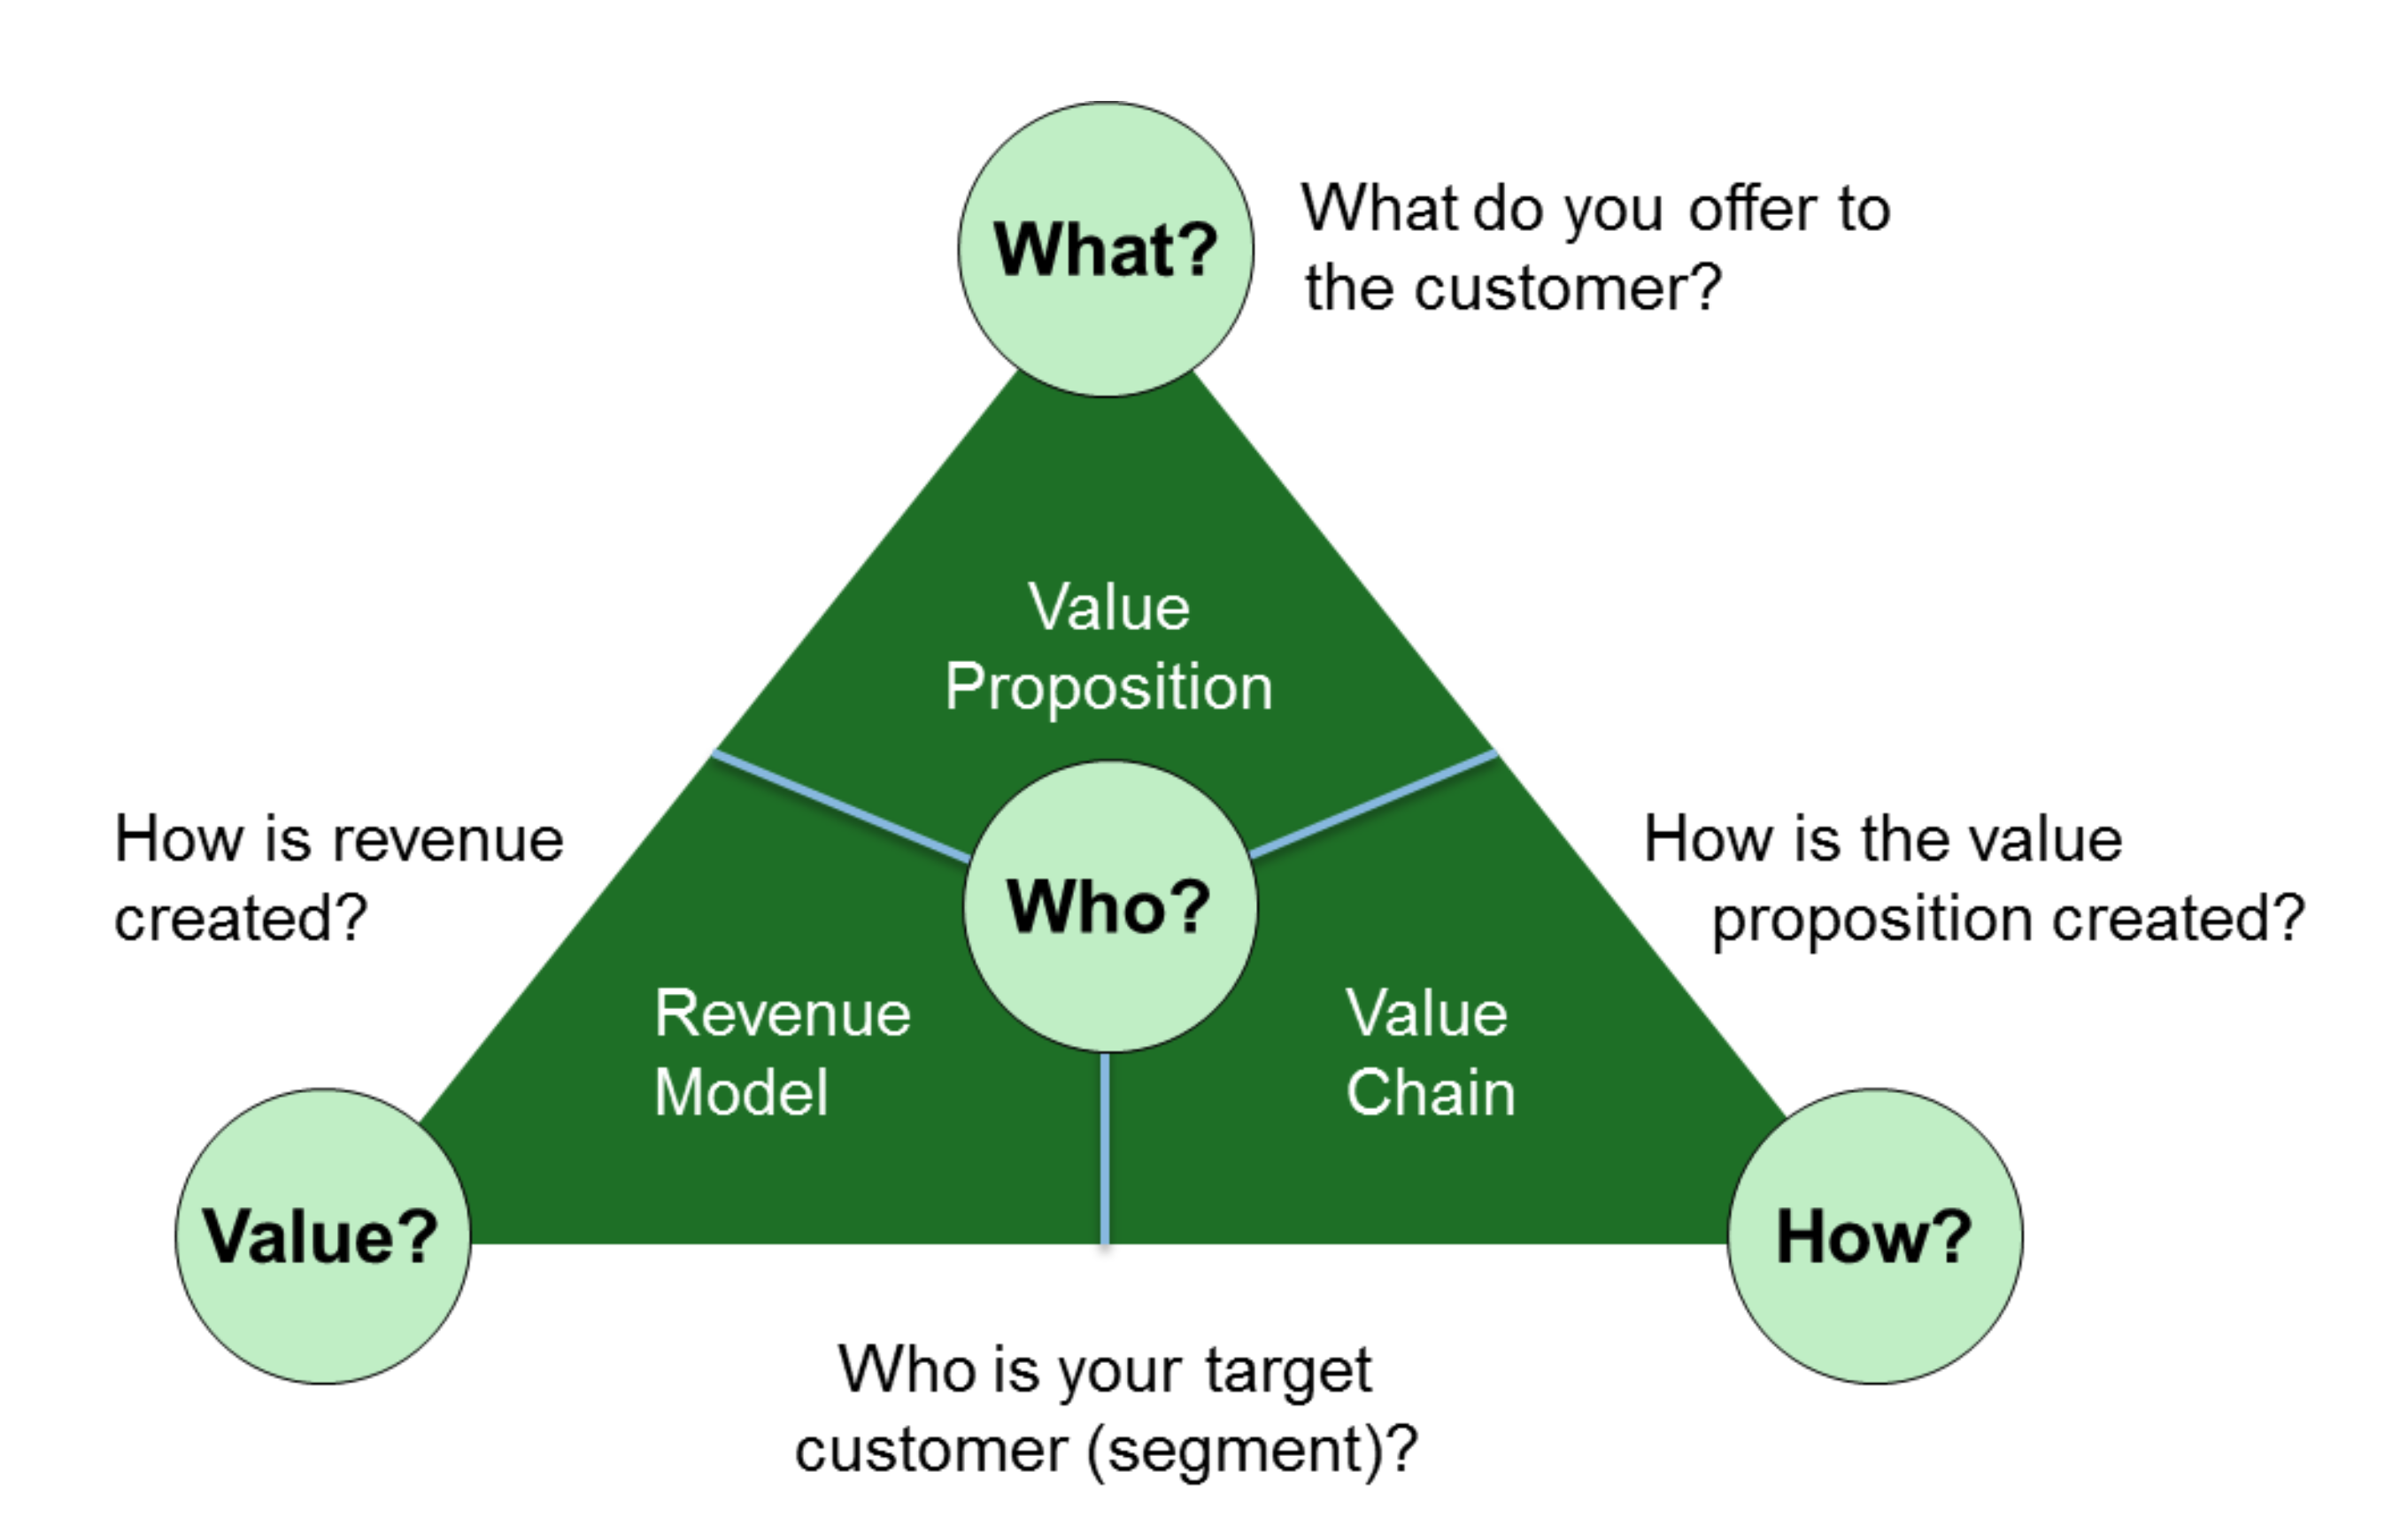
\includegraphics[width=1\columnwidth]{images/BMN}
\caption{Business Model definition - the magic triangle from \citeauthor{gassmann:gallen:2013geschaeftsmodelle}}
\label{fig:BMN}
\end{figure}

%TODO PB St Gallen und MIT Buch einfügen

\subsubsection{Leading Digital}

Technology, operations and business model have been covered, but a business is also strongly influenced by its culture which in turn is strongly influenced by its leadership. While the \ac{WEF} recommends adapting a business culture and focusing on \emph{"attracting and retaining talent in the digital age"}\cite{worldforumdigitalenterprise:2016}, it focuses on attracting millennials and developing the workforce from a human resources perspective. During our literature research we found surprisingly little on the development of corporate culture in regards to \ac{I4.0} and \ac{DT}. \citeauthor{hammer:2015} performed a number of interviews, collecting recommendations by industry experts with an average of 17 years of work experience, summarising the responses with recommendations for more \emph{"trial \& error environments, more employee freedoms, less hierarchy and a two-world IT"}. \citeauthor{bonnect2014leading} encourage a top down approach for shaping a companies culture by communicating goals clearly and often, have the management lead the way in the digital engagement, find digital champions in an organization and amplify their network impact and finally identify quick wins to affirm the strategy of transformation by showing results fast. 


%\subsection{Terminology}

%\begin{itemize}
%\item
%what is Industrie 4.0 in relation to other words in the english-speaking environment
%\item
%does Industrie 4.0 also apply to industries that aren't involved in manufacturing
%\end{itemize}

%Compare to
%\cite{Wirtschaft_en:2016}
%and \cite{Wirtschaft:2016}
%for how the official translation handles the terms
